La placa es de una sola cara, de $190{,}5\times139{,}7$~mm, para una baquela de $20\times15$~cm (Figs.~\ref{fig:pcb_ens} y \ref{fig:pcb_cu}). Se generó con un programa propio en Python, el mismo usado para las tarjetas PID~\cite{informepid}: colocación por recocido simulado dentro de regiones por etapa y ruteo negociado. Las reglas de diseño son:
\begin{itemize}
\item Pistas de 0,8~mm, y de 1,6~mm para las redes de corriente alta: secundario, $V_{RAW\pm}$, emisores y colectores de los transistores de paso, salidas $\pm16$~V y GND. Con cobre de 35~µm, 1,6~mm conducen unos 3~A con 10~°C de aumento.
\item Pads de 2,0~mm, y de 2,6~mm en borneras, portafusibles, diodos 1N5408, $R_{SC}$ y capacitores grandes.
\item Separación mínima entre redes de 0,40~mm, verificada sobre la geometría final.
\end{itemize}
Las 32 redes quedan completas, sin cortos, y el esquemático y la placa son consistentes. Hay siete puentes de alambre del lado de componentes (P1--P7, lista en \texttt{puentes.md}), todos en redes de señal o de baja corriente.

Los cuatro semiconductores de potencia de cada riel van alineados en un borde con la aleta hacia afuera: $Q_1$, $Q_2$, $Q_4$ y U1 arriba, y $Q_5$, $Q_6$, $Q_8$ y U2 abajo. Así se atornillan a un solo disipador por riel. Los capacitores de filtro están en el borde izquierdo y las borneras de salida (J2, J4, J5) en el derecho. En las esquinas hay cuatro agujeros de montaje de 3,2~mm.

En la carpeta \texttt{fuente/hardware/pcb/} están:
\begin{itemize}
\item \texttt{fuente.sch} y \texttt{fuente.brd}, en formato EAGLE, que Fusion Electronics abre.
\item \texttt{cobre\_espejado\_1a1.pdf}: el cobre espejado a escala 1:1, con una regla de 50~mm para comprobar la escala.
\item \texttt{ensamble\_1a1.pdf}: vista de componentes a 1:1 y una vista ampliada con valores.
\item \texttt{puentes.md}: la lista de los siete puentes.
\end{itemize}

\begin{figure*}[!t]
\centering
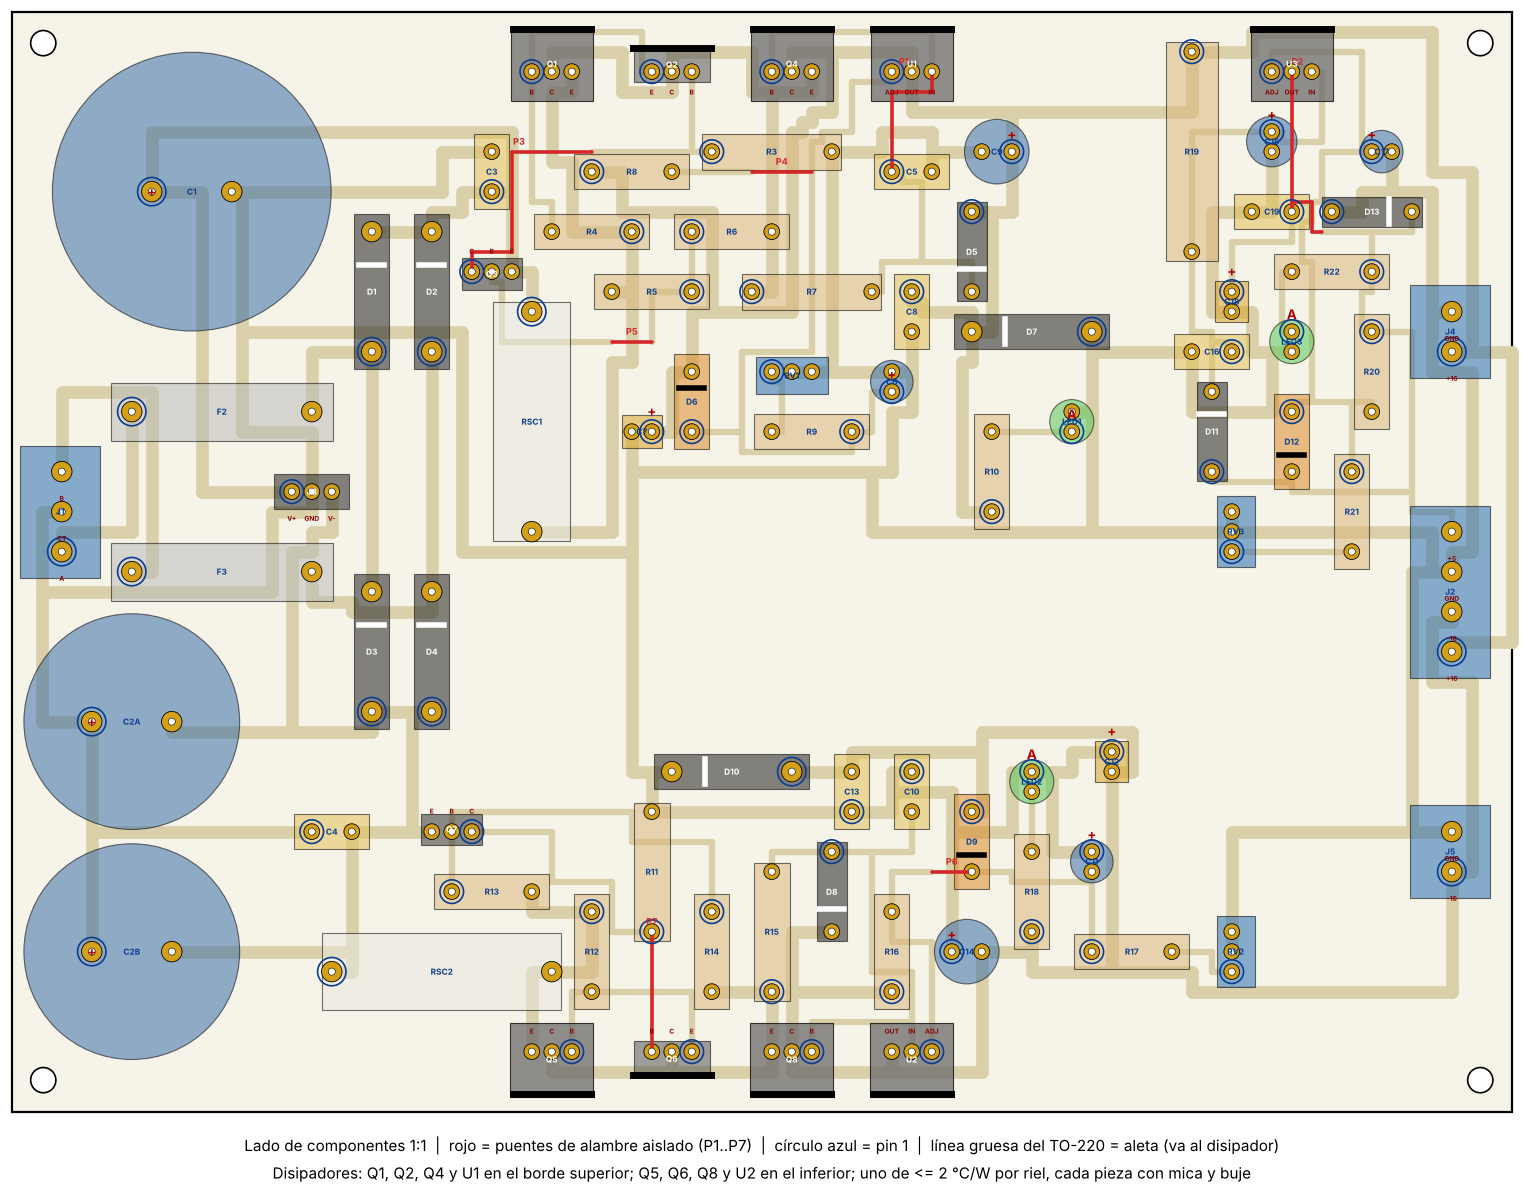
\includegraphics[width=0.9\textwidth]{pcb_ensamble.png}
\caption{Vista de ensamble (lado de componentes). Rojo: puentes de alambre P1--P7. Línea gruesa de cada TO-220/TO-126: aleta, que va al disipador. Círculo azul: pin~1.}
\label{fig:pcb_ens}
\end{figure*}

\begin{figure}[htbp]
\centering
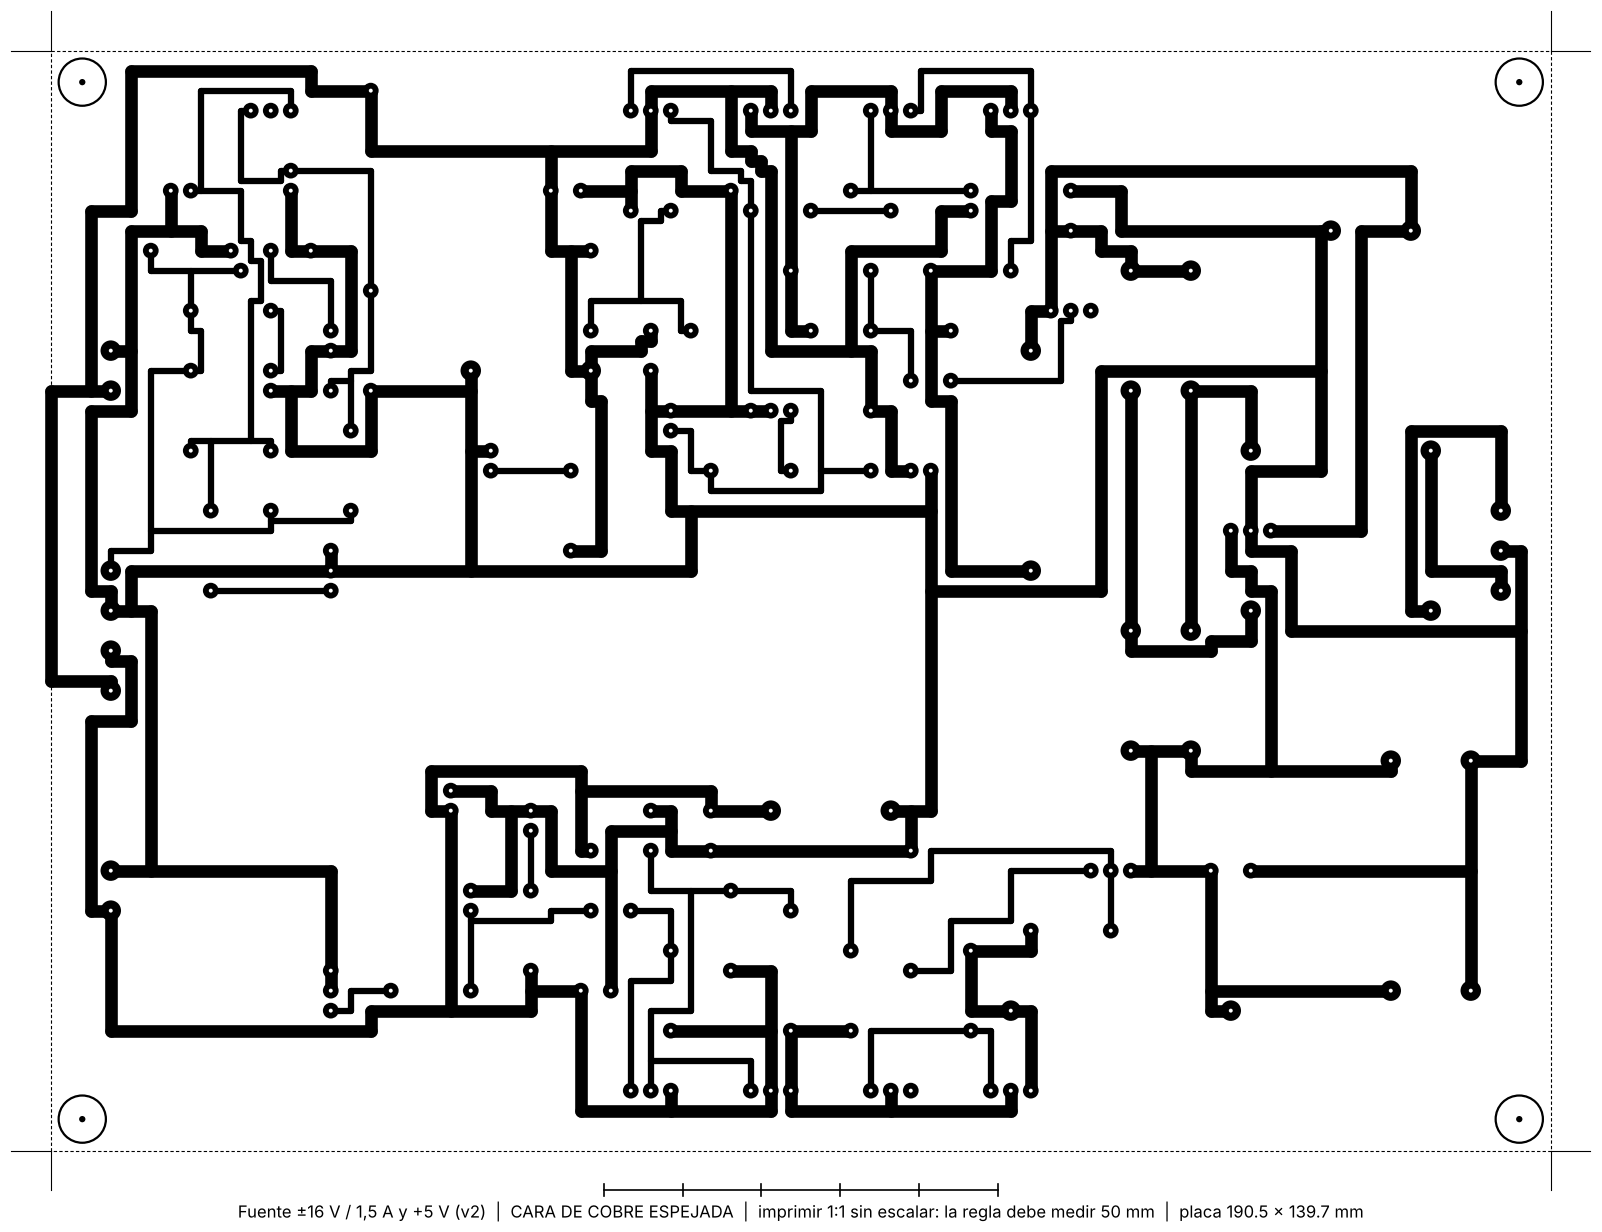
\includegraphics[width=\linewidth]{pcb_cobre_espejado.png}
\caption{Cara de cobre espejada (reducida; la hoja para imprimir es la de 1:1).}
\label{fig:pcb_cu}
\end{figure}

\subsection{Guía de conexión}
La Tabla~\ref{tab:conex} indica cómo se conecta la fuente. Las salidas de J2 llevan el mismo orden que \texttt{J\_PWR} de las tarjetas PID, así que basta un cable de cuatro hilos a una tarjeta, y de ella a la otra. La carga de prueba $R_L$ se atornilla en J4 o J5 solo durante la prueba de 1,5~A, y se retira para medir sin carga o para alimentar los PID. La fuente de las bobinas va por separado a \texttt{J\_VBOB}, y GND con PGND se unen solo en un \texttt{JP\_GND}.

\begin{table}[htbp]
\caption{Guía de conexión}
\label{tab:conex}
\centering
\footnotesize
\begin{tabular}{@{}p{0.42\linewidth}p{0.48\linewidth}@{}}
\toprule
Desde & Hacia \\
\midrule
Red L $\rightarrow$ F1 T1~A $\rightarrow$ S1 & Primario del transformador \\
Red N & Otro extremo del primario \\
Secundario: extremo A / toma central / extremo B & J1-1 / J1-2 (GND) / J1-3 \\
J2-1/2/3/4 (+16, $-16$, GND, +5) & \texttt{J\_PWR} 1/2/3/4 de la tarjeta PID A; de A a B por su \texttt{J\_PWR} \\
J4-1 (+16) y J4-2 (GND) & $R_L=\SI{10}{\ohm}$, $\geq$30~W, removible \\
J5-1 ($-16$) y J5-2 (GND) & $R_L$, removible (un riel a la vez) \\
J3 ($V_{RAW+}$, GND, $V_{RAW-}$) & Osciloscopio (rizado) \\
Disipador superior ($\leq$2~°C/W) & $Q_1$, $Q_2$, $Q_4$ y U1, con mica y buje \\
Disipador inferior ($\leq$2~°C/W) & $Q_5$, $Q_6$, $Q_8$ y U2, con mica y buje \\
\bottomrule
\end{tabular}
\end{table}
